\problemname{High Noon}

Gör det redo, cowboy. 

Du har en duell vid high noon (klockan 12 mitt på dagen). 
Se till att vara här i tid för att skjuta ditt skott.

\begin{centering}
  \begin{figure}[h]
      \centering
      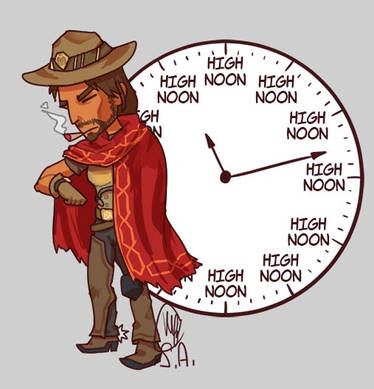
\includegraphics[width=0.8\textwidth]{highnoon.jpg}
      \caption{"Local Man Tells the Time" av essuei, från \href{https://www.deviantart.com/essuei/art/Overwatch-Local-Man-Tells-the-Time-614496598}{www.deviantart.com}. Licenserat under \href{https://creativecommons.org/licenses/by-nc-nd/3.0/}{CC BY-NC-ND 3.0 DEED}.}
  \end{figure}
\end{centering}

\section*{Indata}
Det finns ingen indata. Se bara till att du är redo.

\section*{Utdata}
Skriv ut ``PANG!'' på en rad för att skjuta ditt skott.

\section*{Poängsättning}
\textbf{Notera:} Du kan endast submitta \textbf{en} korrekt lösning för detta problem. Om du redan har submittat en korrekt lösning kommer endast den första att räknas.  
Du kan få 0 till 100 poäng. Om du submittar precis vid \href{https://www.timeanddate.com/worldclock/fixedtime.html?msg=Ready+yourself%2C+Cowboy&iso=20240401T12&p1=239}{High Noon} 
($12:00:00$ Svensk tid), får du exakt 100 poäng. För varje sekund ifrån $12:00:00$ du submittar, får du 1 poäng mindre. 

Till exempel om du submittar vid $11:59:55$ får du endast $95$ poäng. Om du submittar $12:01:00$ får du endast $40$ poäng.
Men om du submittar $11:30:00$ kommer du få $0$ poäng.
